\section{Algorithm}
\nblink{brats/16\_brats\_hausdorff\_masks\_examples.ipynb}
\nblink{brats/24\_testnet\_hdm\_analyze.ipynb}

doc: describe bug with hausdorff distance

check 1: this increases the performance!

\begin{figure}[H]
    \centering
    \begin{subfigure}{.33\textwidth}
        \centering
        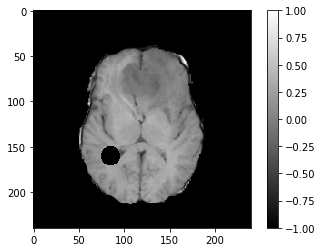
\includegraphics[width=\linewidth]{chapters/06_hdm/images_masked/masked_0.png}
        \caption{T1 modality with mask applied}
    \end{subfigure}%
    \begin{subfigure}{.33\textwidth}
        \centering
        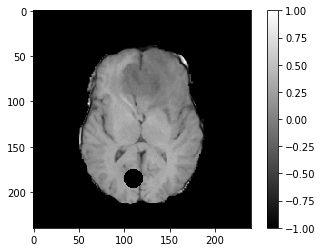
\includegraphics[width=\linewidth]{chapters/06_hdm/images_masked/masked_4.png}
        \caption{T1 modality with a different mask applied}
    \end{subfigure}
        \begin{subfigure}{.33\textwidth}
        \centering
        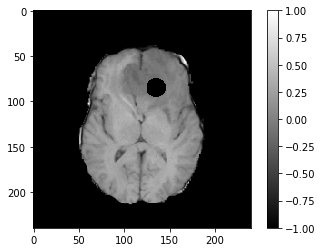
\includegraphics[width=\linewidth]{chapters/06_hdm/images_masked/masked_8.png}
        \caption{T1 modality with a third mask applied}
    \end{subfigure}
    \caption{Modality T1 with three different round masks applied}
\end{figure}

\begin{figure}[H]
    \centering
    \begin{subfigure}{.33\textwidth}
        \centering
        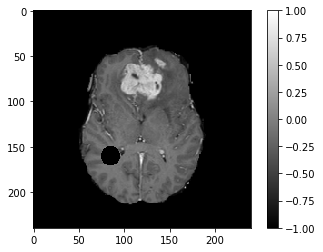
\includegraphics[width=\linewidth]{chapters/06_hdm/images_masked/masked_1.png}
        \caption{T1 enhanced contrast modality with mask applied}
    \end{subfigure}%
    \begin{subfigure}{.33\textwidth}
        \centering
        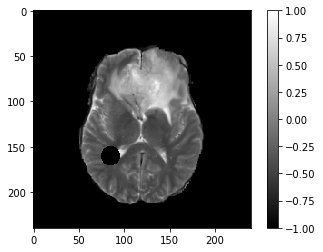
\includegraphics[width=\linewidth]{chapters/06_hdm/images_masked/masked_2.png}
        \caption{T2 modality with mask applied}
    \end{subfigure}
        \begin{subfigure}{.33\textwidth}
        \centering
        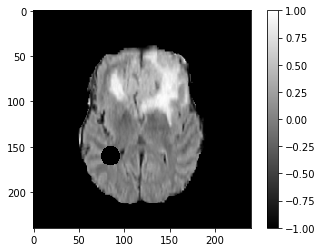
\includegraphics[width=\linewidth]{chapters/06_hdm/images_masked/masked_3.png}
        \caption{FLAIR modality with mask applied}
    \end{subfigure}
    \caption{Modalities T1 contrast enhanced, T2 and FLAIR with the same mask applied}
\end{figure}

